
\section{Engineered system}
\label{chapter-scenario-template}

\textbf{Created by:}  \\
\textbf{Modified by:}  \\

\subsection*{Scenario Objective}
In the IOF Core, a system is defined as a collection of elements. The IOF Core also introduces the notion of an engineered system as an extension of system, which can be used to classify a wide range of industrial systems. While systems, like artifacts, may have parts, properties, roles, and capabilities, unlike material artifacts, which are objects, the systems is classified as BFO’s `object aggregate' rather than object. This modeling choice provides a unique opportunity to capture nuanced semantics regarding the components structure of industrial systems. The following pattern illustrates key aspects of the IOF Core’s system class.

\subsection*{General Pattern Description}

\textit{Important points to discuss}:

\begin{enumerate}
    \item System as object aggregate, it can have components as members (member of) or part (cont. part of).
    \item System components can be both artifacts and sun-system (another system).
    \item Engineered system has designed function that is prescribed by a designed specification.  
    \item System components have their function which are part of the function of the system as a whole.
    \item system and its components can be product (product role) or equipment (equipment role).
\end{enumerate}


\subsection*{Use Case: Mazak machine and its components}
 \textit{Mazak machine with some subsystems and artifacts as component.}

\subsubsection*{Use-Case Pattern Description}

\textit{Mazak machine with 2/3 system components with one of them having their components and 2/3 material artifacts as components. Some of these components should have their functions as part of the function of the system. Additionally various qualities may also be asserted as examples.}

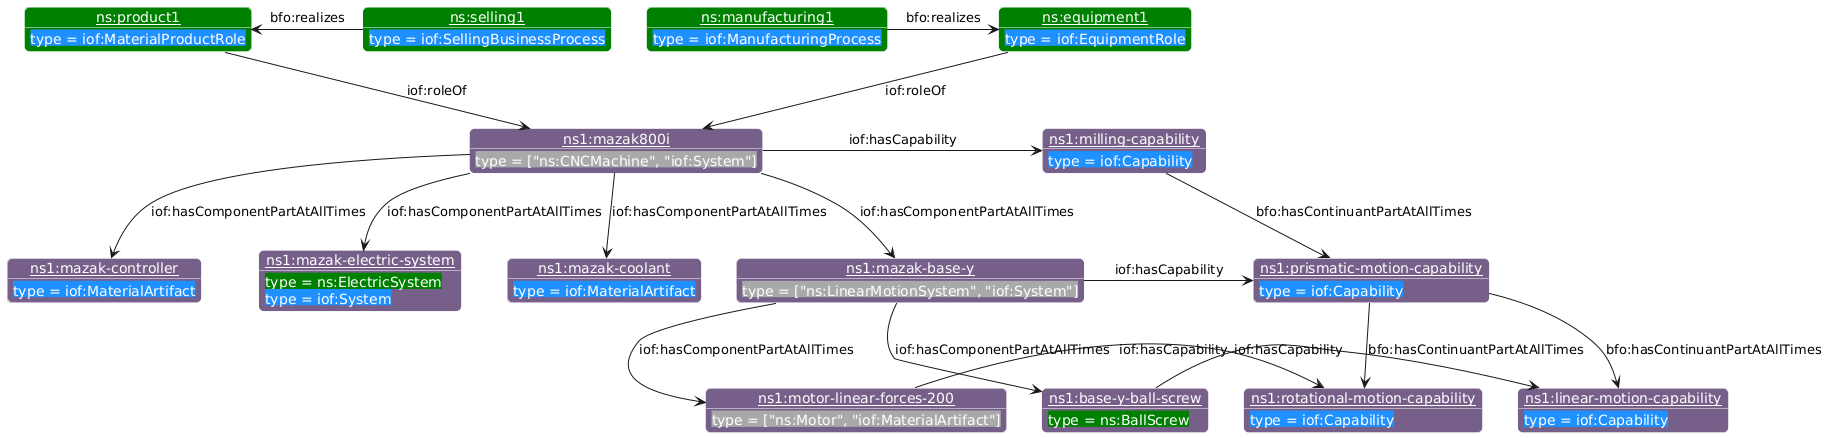
\includegraphics[scale=0.26]{scenarios/engineered-system-artifact/images/mazak.png}
 
\textit{Mazak machine can have different roles, e.g., the machine is sold by Mazak. In a factory, the machine is used to cut metal parts, where it has equipment role (this may be a separate use case).}

\textit{Another aspect is that the mazak machine is prescribed by a corresponding design specification, which also can be in a separate use case}

\subsubsection*{Use-Case Example Data}

\subsubsection*{Data Mapping}
 \textit{ 
Describe how the data was mapped to RDF. Provide an INSERT DATA/ INSERT SPARQL for mapping. Use INSERT only when the use case example data needs further manipulation. \\
For INSERT DATA SPARQL, use only 2/3 records/transactions with named class and individuals. \\
For INSERT SPARQL, declare column names by `\{ \}' to the variable.  
For INSERT query, 
For both, do not use blank nodes.    
  }

\subsubsection*{Data Validation}
 \textit{ 
Data validation can be performed in two ways: accessing interesting facts using SPARQL or validating whether the entire data conforms to the ontology using SHACL. It is preferable to provide both. \\
Provide the SPARQL query in the code block along with the result of the query. \\
  }